%----------------------------------------------------------------------------------------
%	PACKAGES AND THEMES
%----------------------------------------------------------------------------------------

\documentclass[table]{beamer}

\mode<presentation> {

% The Beamer class comes with a number of default slide themes
% which change the colors and layouts of slides. Below this is a list
% of all the themes, uncomment each in turn to see what they look like.

%\usetheme{default}
%\usetheme{AnnArbor}
%\usetheme{Antibes}
%\usetheme{Bergen}
\usetheme{Berkeley}
%\usetheme{Berlin}
%\usetheme{Boadilla}
%\usetheme{CambridgeUS}
%\usetheme{Copenhagen}
%\usetheme{Darmstadt}
%\usetheme{Dresden}
%\usetheme{Frankfurt}
%\usetheme{Goettingen}
%\usetheme{Hannover}
%\usetheme{Ilmenau}
%\usetheme{JuanLesPins}
%\usetheme{Luebeck}
%\usetheme{Madrid}
%\usetheme{Malmoe}
%\usetheme{Marburg}
%\usetheme{Montpellier}
%\usetheme{PaloAlto}
%\usetheme{Pittsburgh}
%\usetheme{Rochester}
%\usetheme{Singapore}
%\usetheme{Szeged}
%\usetheme{Warsaw}

% As well as themes, the Beamer class has a number of color themes
% for any slide theme. Uncomment each of these in turn to see how it
% changes the colors of your current slide theme.

%\usecolortheme{albatross}
%\usecolortheme{beaver}
%\usecolortheme{beetle}
%\usecolortheme{crane}
%\usecolortheme{dolphin}
%\usecolortheme{dove}
%\usecolortheme{fly}
%\usecolortheme{lily}
%\usecolortheme{orchid}
%\usecolortheme{rose}
%\usecolortheme{seagull}
%\usecolortheme{seahorse}
%\usecolortheme{whale}
%\usecolortheme{wolverine}

%\setbeamertemplate{footline} % To remove the footer line in all slides uncomment this line
%\setbeamertemplate{footline}[page number] % To replace the footer line in all slides with a simple slide count uncomment this line

%\setbeamertemplate{navigation symbols}{} % To remove the navigation symbols from the bottom of all slides uncomment this line
}

\usepackage{graphicx} % Allows including images
\usepackage{epstopdf}
\usepackage{booktabs} % Allows the use of \toprule, \midrule and \bottomrule in tables
\usepackage{multirow}
\usepackage[export]{adjustbox}
\usepackage{gensymb}
\renewcommand\footnoterule{{\color{black}\hrule height 0pt}}
\usepackage{appendixnumberbeamer} 
\usepackage{textgreek}
\usepackage{xcolor}
\usepackage{colortbl}
\usepackage{gensymb}
\graphicspath{{pics}}
\usepackage[normalem]{ulem}
\usepackage{mathtools}
\usepackage{amsmath}
\usepackage{amsfonts}

\newcommand{\overbar}[1]{\mkern 1.5mu\overline{\mkern-1.5mu#1\mkern-1.5mu}\mkern 1.5mu}

\setbeamertemplate{caption}{\raggedright\insertcaption\par}
\setbeamertemplate{navigation symbols}{}
\setbeamertemplate{itemize items}[circle]

\usepackage[absolute,overlay]{textpos}

%\AtBeginSection{\frame{\sectionpage}}

%----------------------------------------------------------------------------------------
%	TITLE PAGE
%----------------------------------------------------------------------------------------

\title[GREAT-NS Lecture 7]{Isotopes and the Chart of Nuclides} % The short title appears at the bottom of every slide, the full title is only on the title page

\author{Fatima H. Garcia} % Your name
\institute[GREAT-NS] % Your institution as it will appear on the bottom of every slide, may be shorthand to save space
{
} % Date, can be changed to a custom date
\date{March 8th, 2022}

\begin{document}

\section{Elements vs Isotopes}
\begin{frame}
\titlepage % Print the title page as the first slide
\end{frame}

\begin{frame}
\begin{figure}
\includegraphics[width=\textwidth]{IntroSlide.png}
\end{figure}
\end{frame}

\section{Periodic table vs Chart of Nuclides}
\begin{frame}
\frametitle{Chemistry: the periodic table}
It sorts the known elements into periods (rows) and groups (columns) with similar properties
\begin{figure}
\center
\includegraphics[width=0.9\textwidth]{Periodic-table.jpg}
\end{figure}
\let\thefootnote\relax\footnote{\tiny{Chemistry Learner: https://www.chemistrylearner.com/the-periodic-table}}
\end{frame}

\begin{frame}
\frametitle{Groups: the alkalis}
\begin{figure}
\includegraphics[width=0.9\textwidth]{Alkalis.png}
\end{figure}
These elements have one extra electron, ready to be donated. Pretty reactive; the metallic elements will explode on contact with water
\let\thefootnote\relax\footnote{\tiny{Chemistry Learner: https://www.chemistrylearner.com/the-periodic-table}}
\end{frame}

\begin{frame}
\frametitle{Groups: the halogens}
\begin{figure}
\includegraphics[width=0.9\textwidth]{Halogens.png}
\end{figure}
Also pretty reactive, these elements need one more electron to close their shells. 
\let\thefootnote\relax\footnote{\tiny{Chemistry Learner: https://www.chemistrylearner.com/the-periodic-table}}
\end{frame}

\begin{frame}
\frametitle{Groups: the noble gases}
\begin{figure}
\includegraphics[width=0.9\textwidth]{NobleGases.png}
\end{figure}
These elements have a full complement of electrons and therefore are not keen on interacting with anything. 
\let\thefootnote\relax\footnote{\tiny{Chemistry Learner: https://www.chemistrylearner.com/the-periodic-table}}
\end{frame}

\section{History Detour}

\begin{frame}
\frametitle{The key distinction}
The introduction of the neutron meant that a new classification system was required \\
Short detour: the discovery of the protons and the term 'isotope'
\vspace{10pt}
\begin{columns}[c]
\column{0.3\textwidth}
Soddy:
\begin{figure}
\includegraphics[width=0.7\textwidth]{Soddy.jpeg}
\end{figure}
\column{0.3\textwidth}
Chadwick:
\begin{figure}
\includegraphics[width=0.8\textwidth]{Chadwick.jpeg}
\end{figure}
\column{0.3\textwidth}
Segr\`{e}
\begin{figure}
\includegraphics[width=0.7\textwidth]{Segre.jpeg}
\end{figure}
\end{columns}
\let\thefootnote\relax\footnote{\tiny{https://en.wikipedia.org/wiki/Frederick\_Soddy}}
\let\thefootnote\relax\footnote{\tiny{https://en.wikipedia.org/wiki/Discovery\_of\_the\_neutron}}
\let\thefootnote\relax\footnote{\tiny{https://en.wikipedia.org/wiki/Emilio\_Segr\`{e}}}
\end{frame}

\begin{frame}
\frametitle{Radioelements and the term 'Isotope'}
Frederick Soddy
\begin{columns}[c]
\column{0.3\textwidth}
\begin{figure}
\includegraphics[width=\textwidth]{Soddy.jpeg}
\end{figure}
\column{0.7\textwidth}
\begin{itemize}
\item Discovered that radium is a daughter of uranium decay
\item Showed that one radioactive element might have more than one atomic mass but exhibit the same chemical properties
\item Coined the term 'isotope': meaning same place
\item Was awarded the Nobel prize in Chemistry in 1921
\end{itemize}
\end{columns}
\vspace{10pt}
Fun fact: developed an economic model based around physics? The economists thought he was crazy
\let\thefootnote\relax\footnote{\tiny{https://cen.acs.org/articles/91/i48/Celebrating-Isotope.html}}
\end{frame}

\begin{frame}
\frametitle{The discovery of the neutron}
James Chadwick
\begin{columns}[c]
\column{0.3\textwidth}
\begin{figure}
\includegraphics[width=\textwidth]{Chadwick.jpeg}
\end{figure}
\column{0.7\textwidth}
\begin{itemize}
\item Worked alongside Rutherford at the Cavendish Lab
\item In 1932 (after only two weeks!) he had a paper on the neutron (a more formal one followed months after
\item Photodisintegration of deuterium: $^{2}_{1}\texttt{D} + \gamma \rightarrow \texttt{ } ^{1}_{1}\texttt{H} + \texttt{n}$
\item Was awarded the Nobel Prize Physics in 1935
\end{itemize}
\end{columns}
\vspace{10pt}
Fun fact: He was head of the college that Francis Crick attended when he and Watson 'discovered' the structure of DNA
\let\thefootnote\relax\footnote{\tiny{https://www.aps.org/publications/apsnews/200705/physicshistory.cfm}}
\end{frame}

\begin{frame}
\frametitle{The new 'periodic table'}
\begin{columns}[c]
\column{0.3\textwidth}
\begin{figure}
\includegraphics[width=\textwidth]{Segre.jpeg}
\end{figure}
\column{0.7\textwidth}
\begin{itemize}
\item Discovered technicium (first element with no stable isotopes) and astatine
\item Published a detailed chart of nuclides in 1946
\item Worked extensively at LBNL where he discovered the antiproton
\item Was awarded the Nobel Prize in Physics in 1959 (jointly with Owen Chamberlain) for the discovery of the antiproton
\end{itemize}
\end{columns}
\let\thefootnote\relax\footnote{\tiny{https://www.nap.edu/read/10470/chapter/18\#299}}
\end{frame}

\begin{frame}
\frametitle{The Chart of Nuclides}
The periodic table for nuclear science; arranging isotopes by their proton and neutron numbers
\begin{figure}
\includegraphics[width=0.9\textwidth]{NNDCChart.png}
\end{figure}
\let\thefootnote\relax\footnote{\tiny{NNDC: https://www.nndc.bnl.gov/nudat3/nudat2.jsp}}
\end{frame}

\begin{frame}
\frametitle{The Chart of Nuclides}
\begin{figure}
\includegraphics[width=0.9\textwidth]{Chart1.png}
\end{figure}
\let\thefootnote\relax\footnote{\tiny{NNDC: https://www.nndc.bnl.gov/nudat3/nudat2.jsp}}
\end{frame}

\begin{frame}
\frametitle{The Chart of Nuclides}
\begin{figure}
\includegraphics[width=0.9\textwidth]{Chart2.png}
\end{figure}
\let\thefootnote\relax\footnote{\tiny{NNDC: https://www.nndc.bnl.gov/nudat3/nudat2.jsp}}
\end{frame}

\begin{frame}
\frametitle{The Chart of Nuclides}
\begin{figure}
\includegraphics[width=0.9\textwidth]{Chart3.png}
\end{figure}
\let\thefootnote\relax\footnote{\tiny{NNDC: https://www.nndc.bnl.gov/nudat3/nudat2.jsp}}
\end{frame}

\begin{frame}
\frametitle{The Chart of Nuclides}
\begin{figure}
\includegraphics[width=0.9\textwidth]{Chart4.png}
\end{figure}
\let\thefootnote\relax\footnote{\tiny{NNDC: https://www.nndc.bnl.gov/nudat3/nudat2.jsp}}
\end{frame}

\section{Notation}
\begin{frame}
\frametitle{Reading the chart}
The periodic table gives you information about the element, such as atomic weight, and the atomic number (this is the number of protons)
\begin{figure}
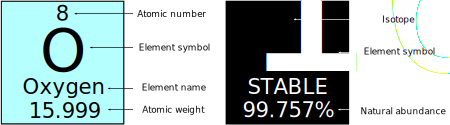
\includegraphics[width=\textwidth]{ElementvsIsotopeSymbol.png}
\end{figure}
The chart of nuclides gives you information about the number protons and neutrons, the 'stability' of the nucleus and in the case of stable isotopes, the natural abundance of each isotope
\end{frame}

\begin{frame}
\frametitle{Different isotopes}
The chart also gives you information about isotope decay, half-life and branching ratios
\begin{figure}
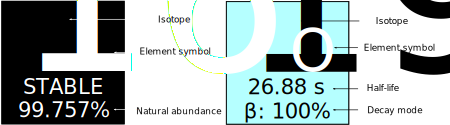
\includegraphics[width=\textwidth]{OxygenIsotopes.png}
\end{figure}
Quick question: How many neutrons does $^{19}$O have?
\end{frame}

\begin{frame}
\frametitle{Different isotopes}
The chart also gives you information about isotope decay, half-life and branching ratios
\begin{figure}
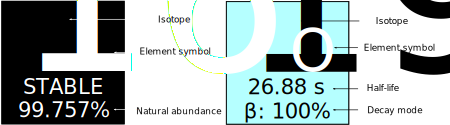
\includegraphics[width=\textwidth]{OxygenIsotopes.png}
\end{figure}
Quick question: How many protons and how many neutrons does $^{19}$O have? \\
\textcolor{blue}{8 protons, 11 neutrons}
\end{frame}

\begin{frame}
\frametitle{Unstable isotopes}
\begin{columns}[c]
\column{0.5\textwidth}
\begin{figure}
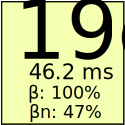
\includegraphics[width=0.7\textwidth]{Carbon19.png}
\end{figure}
\column{0.5\textwidth}
\end{columns}
\end{frame}

\begin{frame}
\frametitle{Unstable isotopes}
\begin{columns}[c]
\column{0.5\textwidth}
\begin{figure}
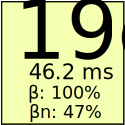
\includegraphics[width=0.7\textwidth]{Carbon19.png}
\end{figure}
\column{0.5\textwidth}
\begin{itemize}
\item 13 neutrons (compared to the 6 neutrons $^{12}$C has)
\item Short half-life (milliseconds)
\item Decays through $\beta$-decay
\item Also decays through $\beta$-delayed neutron emission
\end{itemize}
\end{columns}
\end{frame}

\section{Isotopes, isobars and isotones}
\begin{frame}
\frametitle{Nuclear compass}
\begin{columns}
\column{0.5\textwidth}
\begin{figure}
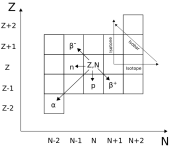
\includegraphics[width=\textwidth]{DecayScheme.png}
\end{figure}
\column{0.5\textwidth}
The positioning of the nuclides along the chart is just as important as the position of the elements on the periodic table.
\vspace{10pt}
Information about decay modes and place in the nuclear landscape.
\end{columns}
\end{frame}


\begin{frame}
\frametitle{Nuclear compass}
\begin{columns}
\column{0.5\textwidth}
\begin{figure}
\includegraphics[width=\textwidth]{DecayScheme-isotope.png}
\end{figure}
\column{0.5\textwidth}
Following the columns, you get isotopes, the same element (proton number) but different neutron numbers
\vspace{10pt} \\
Fun fact: Tin has the largest number of isotopes on the chart
\end{columns}
\end{frame}

\begin{frame}
\frametitle{Nuclear compass}
\begin{columns}
\column{0.5\textwidth}
\begin{figure}
\includegraphics[width=\textwidth]{DecayScheme-isotone.png}
\end{figure}
\column{0.5\textwidth}
Following the columns, you get the same neutron number, but different proton numbers
\vspace{10pt} \\
Fun fact: N=82 is the 'most popular' neutron number
\end{columns}
\end{frame}


\begin{frame}
\frametitle{Nuclear compass}
\begin{columns}
\column{0.5\textwidth}
\begin{figure}
\includegraphics[width=\textwidth]{DecayScheme-isobar.png}
\end{figure}
\column{0.5\textwidth}
Following the diagonal (right to left), you get isobars: isotopes with the same nucleon number, but different combinations of protons and neutrons \\
\vspace{10pt}
Fun fact isobars with swapped proton and neutron numbers are called mirror nuclei: \\
\hspace{1pt} $^{34}_{16}$S$_{18}$ and  $^{34}_{18}$Ar$_{34}$
\end{columns}
\end{frame}

\section{Trends in the chart}
\begin{frame}
\frametitle{Half-life}
\begin{figure}
\includegraphics[width=\textwidth]{HalfLife+Legend.png}
\end{figure}
\end{frame}

\begin{frame}
\frametitle{Decay Modes}
\begin{figure}
\includegraphics[width=\textwidth]{DecayMode+Legend.png}
\end{figure}
\end{frame}

\begin{frame}
\frametitle{Q$_{\beta^{-}}$}
\begin{figure}
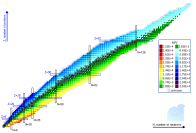
\includegraphics[width=\textwidth]{Qbeta+Legend.png}
\end{figure}
\end{frame}

\begin{frame}
\frametitle{Neutron separation energy}
\begin{figure}
\includegraphics[width=\textwidth]{Sn+Legend.png}
\end{figure}
\end{frame}

\begin{frame}
\frametitle{Q$_{\beta n}$}
\begin{figure}
\includegraphics[width=\textwidth]{BetaDelated+legend.png}
\end{figure}
\end{frame}

\begin{frame}
\frametitle{Excited states: E$_{2^{+}}$}
\begin{figure}
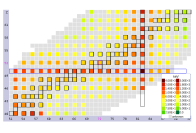
\includegraphics[width=\textwidth]{E2++legend.png}
\end{figure}
\end{frame}


\section{Applications of isotopic properties}
\begin{frame}

\end{frame}

\section{Resources}
\begin{frame}

\end{frame}
 


\end{document} 

